\chapter{Methodology}

\section{Introduction}
\label{sec:methodology_intro}

  For our implementation, we consider an investor holding a long position in a ten-year interest rate swap. This implies that the investor will pay a fixed rate on the notional principal and receive a floating rate referencing the prevailing short-term interest rate, with no exchange of principal and only the net interest cashflow settled between the two parties at each payment date. We assume that the counterparties trade in accordance with the confirmation set out in Table~\ref{tab:swap_confirmation} below, in which Party A is designated the fixed rate payer, corresponding to the investor's long position, and Party B the floating rate payer on the other side of the transaction. \\

  \noindent
    \begin{table}[H]
  \centering
  \caption{Confirmation of the interest rate swap transaction, presented in the format of a standard ISDA confirmation}
  \label{tab:swap_confirmation}
  \begin{tabular}{@{}p{0.38\linewidth}p{0.52\linewidth}@{}}
  \toprule
  \textbf{Field} & \textbf{Value} \\
  \midrule
  \multicolumn{2}{@{}l}{\textit{A. Transaction Details}} \\
  \addlinespace
  Parties                        & Party A and Party B \\
  Trade Date                     & $t = 0$ \\
  Effective Date                 & $t = 0$ \\
  Termination Date               & $T_n = 10$ years from the Effective Date \\
  Calculation Agent              & Party B \\
  \addlinespace
  \multicolumn{2}{@{}l}{\textit{Fixed Amounts}} \\
  \addlinespace
  Fixed Rate Payer               & Party A \\
  Notional Amount                & $N$ (constant; no amortisation) \\
  Fixed Rate                     & $K^{\mathrm{par}}$, set at the Effective Date per the par-swap condition \\
  Fixed Rate Day Count Fraction  & 30/360 (semi-annual accrual, $\tau = 0.5$) \\
  Fixed Rate Payer Payment Dates & $T_j = j\tau$, $j = 1,\dots,20$ (semi-annual, in arrears) \\
  \addlinespace
  \multicolumn{2}{@{}l}{\textit{Floating Amounts}} \\
  \addlinespace
  Floating Rate Payer            & Party B \\
  Notional Amount                & $N$ (matches Fixed Amounts) \\
  Floating Rate Option           & Resets to the instantaneous short rate implied by the
                                    Hull-White model (single-curve valuation, no credit spread) \\
  Spread                         & None \\
  Floating Rate Day Count Fraction & 30/360 (semi-annual accrual, $\tau = 0.5$) \\
  Floating Rate Payer Payment Dates & $T_j = j\tau$, $j = 1,\dots,20$ (semi-annual, in arrears) \\
  Compounding                    & Inapplicable \\
  \addlinespace
  \multicolumn{2}{@{}l}{\textit{Other Terms}} \\
  \addlinespace
  Business Day Convention        & Not applicable (continuous-time model; no calendar
                                    adjustment) \\
  Governing Model                 & One-factor Hull-White short-rate model, calibrated to
                                    the Svensson zero curve at $t = 0$ \\
  \bottomrule
  \end{tabular}
  \end{table}

  \noindent
  We develop and evaluate deep learning surrogate models as replacements for computationally expensive classical pricing routines within a Monte Carlo-based xVA framework. The objective is twofold: to achieve price approximation accuracy that is practically indistinguishable from the underlying Hull-White pricer, and to ensure that the implied price sensitivities are recovered correctly.\footnote{We restrict our attention to the DV01, the sensitivity of the swap value to a parallel shift in the yield curve.} \\

  \noindent
  The first is a standard Gated Recurrent Unit (GRU) network trained on price labels derived from the Hull-White analytical pricer, taking discount factor curves and model parameters as inputs. The second is a differential surrogate trained jointly on price and key-rate DV01 labels, following the differential deep learning framework of \cite{huge2020differential}. The motivation for the comparison is to establish whether joint training on sensitivities produces measurable improvements in both price and Greeks accuracy relative to price-only training.

  \section{Model Assumptions}
  \label{sec:assumptions}


  The analysis rests on a set of modelling assumptions that govern the scope and implementation of this study. These are stated here explicitly to establish a clear theoretical boundary before the technical development begins.\\

  \noindent
  The initial yield curve is parameterised using the Nelson-Siegel-Svensson (1994) functional form, with parameters sourced from the Federal Reserve GSW dataset \cite{gurkaynak2007}. In a practice, the term structure would be
  constructed by bootstrapping from quoted market instruments. The Svensson curves used here serve as analytically smooth proxies, the GSW estimates are fitted daily to US Treasury yields and reproduce the principal shapes observed in real
  fixed income markets, including normal, humped, flat, inverted, and steep configurations. All rates are expressed on a continuously-compounded, act/365 basis. \\

  \begin{figure}[H]
    \centering
    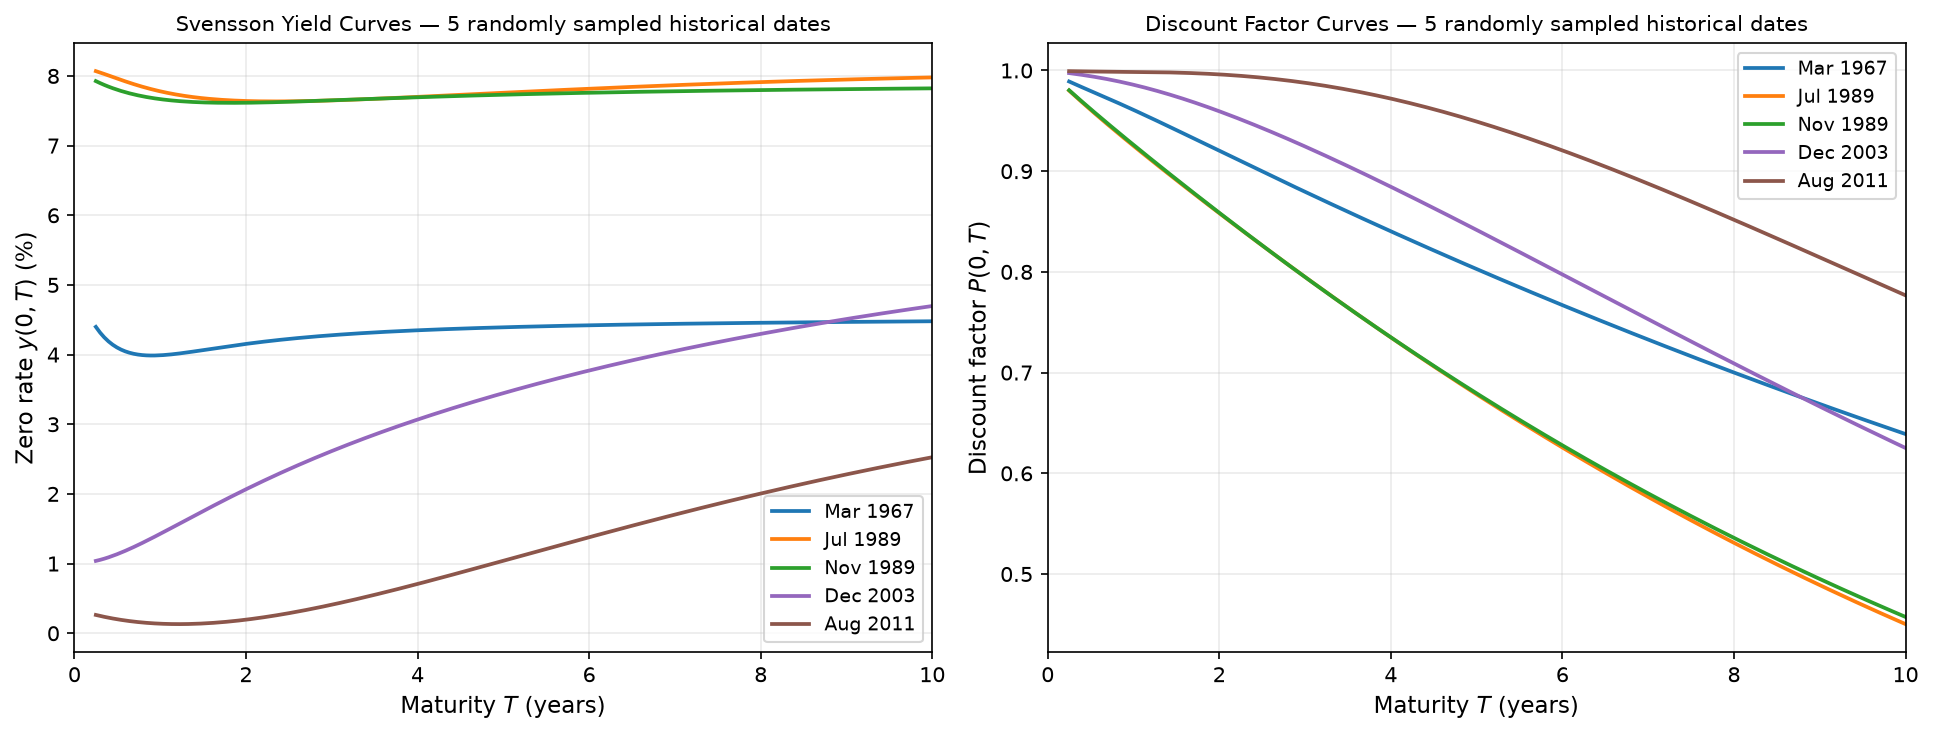
\includegraphics[width=\textwidth]{Images/b1_random_sample.png}
    \caption{Svensson yield curves (left) and corresponding discount factor curves (right)
             for five randomly sampled historical dates from the Federal Reserve GSW dataset.
             The selection illustrates the range of term structure shapes used as proxies
             for market yield curve data in this study.}
    \label{fig:random_sample_curves}
  \end{figure}

  \noindent
  The short rate evolves under the risk-neutral measure $\mathbb{Q}$ according to the Hull-White one-factor dynamics, with mean reversion speed $a > 0$ and instantaneous volatility $\sigma > 0$ both held constant over the full simulation
  horizon. The drift function $\theta(t)$ is uniquely determined by the requirement that the model reproduce the initial term structure exactly. This study does not calibrate $a$ and $\sigma$ from market-implied swaption volatilities, both are instead treated as inputs to the surrogate and sampled across a practical range, enabling the network to approximate the pricing function over a broad region of the parameter space. The simulation is initialised at the instantaneous short rate $r_0 = \lim_{T \to 0} y(0,T) = \beta_0 + \beta_1$, which is the limiting value of the Svensson zero yield as maturity approaches zero \cite{diebold2006forecasting}. \\

  \begin{figure}[H]
    \centering
    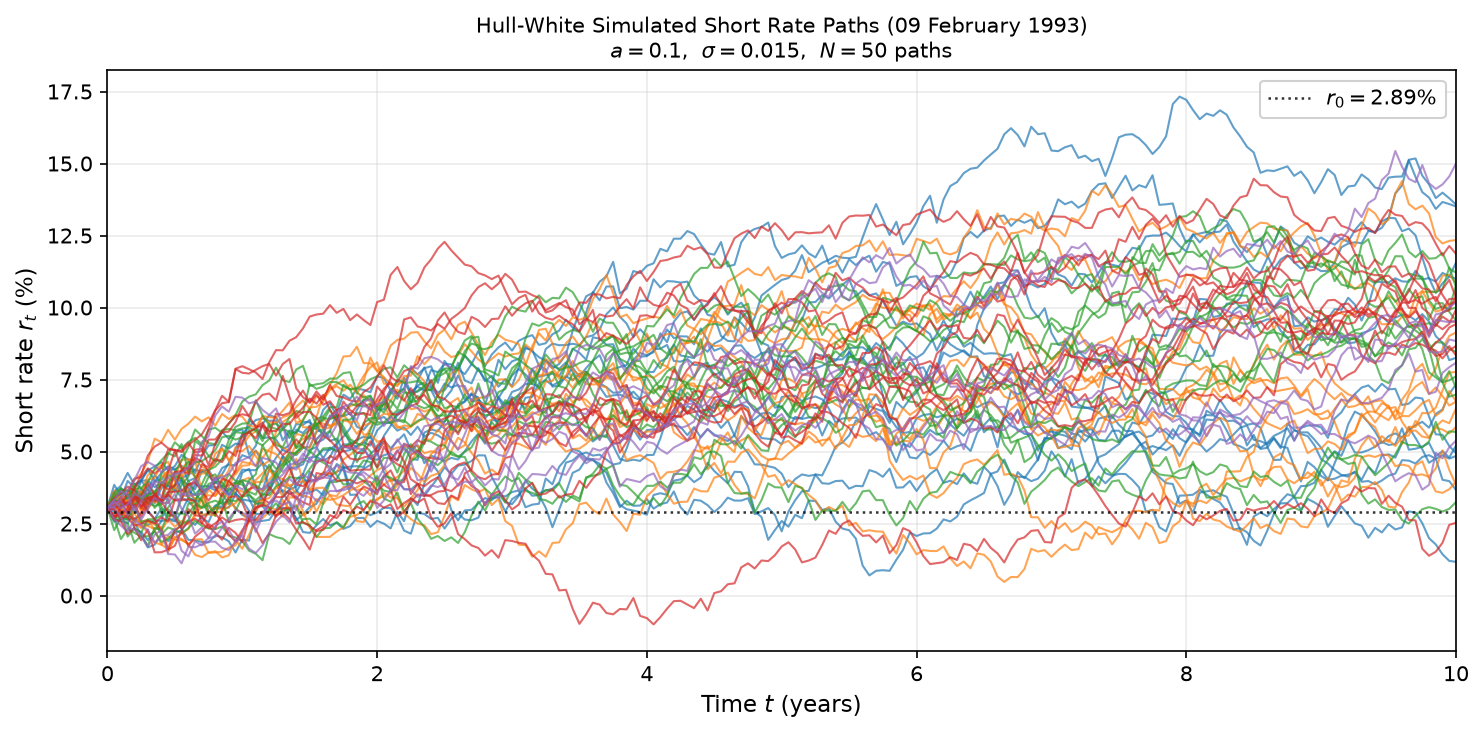
\includegraphics[width=\textwidth]{Images/b1_hw_paths.png}
    \caption{Simulated Hull-White short-rate paths over the ten-year IRS horizon,
             initialised at $r_0 = \beta_0 + \beta_1$ from the Svensson term structure.
             The upward drift of the path ensemble reflects the positive slope of the
             initial forward curve embedded in $\theta(t)$, consistent with an
             upward-sloping initial yield curve.}
    \label{fig:hw_paths}
  \end{figure}

  \noindent
  The underlying instrument is a ten-year payer IRS with semi-annual payment dates $T_j = j\tau$, $j = 1,\ldots,20$, and day count fraction $\tau = 0.5$. A single-curve framework is adopted, the same Svensson-calibrated curve is used for both discounting and floating rate estimation. No credit spread, margin, or collateral agreement is assumed. The swap is initiated at par, so $K = K^{\mathrm{par}}$ and the value at inception is zero. Notional is normalised to $N = 1$, and calendar effects are disregarded throughout. \\

  \noindent
  Monte Carlo simulation is conducted under $\mathbb{Q}$, with the short-rate process discretised via the Euler-Maruyama scheme. The simulation horizon is ten years, divided into 120 monthly steps so that monitoring dates $t_k = k/12$, $k = 0,1,\ldots,120$, align exactly with the path grid. No variance reduction techniques are employed. Training labels for the surrogate models are generated
  analytically from the Hull-White closed-form bond pricing formulae; no simulation noise enters the training data. Sensitivity labels for Model 1b are computed via automatic differentiation, not finite differences. For the xVA calculation, only unilateral CVA is considered, counterparty default is assumed independent of exposure, the hazard rate is flat, and recovery is fixed at $R = 40\%$.



  \section{Numerical Pricing of the IRS Under Hull-White}
  \label{sec:numerical_pricing}

  The computation of Credit Valuation Adjustment requires evaluating the expected positive exposure of the IRS at each date over the full life of the contract. The Expected Positive Exposure at monitoring date $t_k$ is:
  %
  \begin{equation}
    \mathrm{EPE}(t_k)
      = \mathbb{E}^{\mathbb{Q}}\!\left[
          \max\!\bigl(V_{\mathrm{IRS}}(t_k,\,r_{t_k}),\;0\bigr)
        \right]
  \end{equation}
  %
  Computing this across $N$ simulated scenarios and $K = 120$ monthly monitoring dates requires the swap value $V_{\mathrm{IRS}}(t_k, r_{t_k}^{(i)})$ at each scenario $(t_k, r_{t_k}^{(i)})$, for $i = 1,\ldots,N$ and $k = 0,\ldots,120$. This is the central pricing problem: given a future state $(t, r_t)$ with $t > 0$, determine the value of the remaining cashflows of the IRS at that state. \\

  \noindent
  Under the risk-neutral measure $\mathbb{Q}$, this value is the conditional expectation of discounted future net cashflows:
  %
  \begin{equation}
    V_{\mathrm{IRS}}(t, r_t)
      = \mathbb{E}^{\mathbb{Q}}_t\!\left[
          \sum_{j:\,T_j > t}
          \exp\!\left(-\int_t^{T_j} r_s\,\mathrm{d}s\right)\mathrm{CF}_j
        \right]
    \label{eq:rn_pricing}
  \end{equation}
  %
  where $\mathrm{CF}_j$ denotes the net cashflow at payment date $T_j$. Under the Hull-White model, this expectation admits two computationally distinct representations. The first evaluates it in closed form via the affine term structure, yielding an exact analytical price at any $(t, r_t)$. The second estimates it by Monte Carlo simulation, averaging discounted cashflows across forward paths initiated from the state $(t, r_t)$. Both representations evaluate the same expectation; the simulation estimate converges to the analytical price as the number of inner paths increases. \\

  \noindent
  This equivalence motivates the design of the two surrogate models developed in this study. Model 1a is trained to replicate the closed-form pricer, applicable wherever an analytical solution exists. Model 1b is trained to replicate the simulation-based pricer, applicable in the more general setting where no closed form is available, as is the case for multi-factor term structure models or path-dependent payoffs. Since both pricers evaluate the same underlying expectation, their convergence provides a natural validation benchmark: agreement between the two surrogate outputs confirms that each is correctly approximating the same pricing function. The two representations are described in the subsections that follow. \\

  \subsection*{Analytical Valuation: Affine Term Structure}
  \label{sec:affine_pricing}

  The initial discount factors $P(0,T_j)$ at the semi-annual payment dates are computed from the Svensson zero curve:
  %
  \begin{equation}
    P(0, T_j) = \exp\bigl(-y(0, T_j) \cdot T_j\bigr), \quad j = 1,\ldots,20
    \label{eq:df_svensson}
  \end{equation}
  %
  At a future time $t > 0$ and short rate $r_t$, each bond price is computed via the affine formula:
  %
  \begin{equation}
    P(t, T_j) = A(t, T_j)\exp\bigl(-B(t, T_j)\,r_t\bigr)
    \label{eq:hw_bond}
  \end{equation}
  %
  where:
  %
  \begin{align}
    B(t, T_j) &= \frac{1 - e^{-a(T_j - t)}}{a}
    \label{eq:hw_B} \\[4pt]
    \ln A(t, T_j) &= \ln\frac{P(0,T_j)}{P(0,t)}
      - B(t,T_j)\,f(0,t)
      - \frac{\sigma^2}{4a}\,B(t,T_j)^2\bigl(1 - e^{-2at}\bigr)
    \label{eq:hw_A}
  \end{align}
  %
  with $f(0,t)$ the initial instantaneous forward rate, approximated via central differences:
  %
  \begin{equation}
    f(0,t) \approx -\frac{\ln P(0, t+\Delta t) - \ln P(0, t-\Delta t)}{2\Delta t}
    \label{eq:fwd_finite_diff}
  \end{equation}
  %
  The payer IRS value at $(t, r_t)$ is then assembled as:
  %
  \begin{equation}
    V_{\mathrm{IRS}}(t, r_t)
      = P(t, T_0) - P(t, T_n)
        - K^{\mathrm{par}}\,\tau \sum_{j=1}^{n} P(t, T_j)
    \label{eq:irs_value}
  \end{equation}
  %
  with the par rate computed once at $t = 0$:
 
  \subsection*{Simulation-Based Valuation: Monte Carlo}
  \label{sec:mc_pricing}

  The simulation-based representation of \eqref{eq:rn_pricing} estimates the conditional expectation directly by forward simulation. Given a state $(t, r_t)$, $M$ independent short-rate paths are simulated from time $t$ to maturity $T_n$ via the Euler-Maruyama scheme: 
  %
  \begin{equation}
    r_{s+\Delta s}^{(i)}
      = r_s^{(i)}
        + \bigl(\theta(s) - a\,r_s^{(i)}\bigr)\Delta s
        + \sigma\,\sqrt{\Delta s}\,Z_s^{(i)},
    \quad Z_s^{(i)} \sim \mathcal{N}(0,1)
    \label{eq:euler_maruyama}
  \end{equation}
  %
  On each path $i$, the net cashflow at remaining payment date $T_j > t$ is:
  %
  \begin{equation}
    \mathrm{CF}_j^{(i)}
      = \left(\frac{1}{P\!\left(T_{j-1},\,T_j \mid r_{T_{j-1}}^{(i)}\right)} - 1\right)
        - K^{\mathrm{par}}\tau
    \label{eq:mc_cf}
  \end{equation}
  %
  where $P(T_{j-1}, T_j \mid r_{T_{j-1}}^{(i)})$ is the affine bond price
  evaluated at the simulated short rate $r_{T_{j-1}}^{(i)}$. Each cashflow
  is discounted to $t$ using the path numeraire:
  %
  \begin{equation}
    D^{(i)}(t,\,T_j)
      = \exp\!\left(-\sum_{s:\,t \leq s < T_j} r_s^{(i)}\,\Delta s\right)
    \label{eq:path_disc}
  \end{equation}
  %
  The simulation-based swap value is then:
  %
  \begin{equation}
    V_{\mathrm{MC}}(t, r_t)
      = \frac{1}{M}\sum_{i=1}^{M}\;\sum_{j:\,T_j > t}
          \mathrm{CF}_j^{(i)}\,D^{(i)}(t,\,T_j)
    \label{eq:irs_mc}
  \end{equation}
  %
  By the risk-neutral pricing theorem, $V_{\mathrm{MC}}$ is an unbiased estimator of $V_{\mathrm{affine}}$, and the two converge as $M \to \infty$. This is the pricing method replicated by Model 1b.

  \section{Monte Carlo Simulation and Exposure}
  \label{sec:mc_exposure}

  The expected exposure profiles are computed by simulation across $N$
  independent outer paths. For each path $i = 1,\ldots,N$, the short rate
  is evolved from $t = 0$ to $T_n$ via \eqref{eq:euler_maruyama} over
  $K = 120$ monthly monitoring dates $t_k = k/12$, $k = 0,1,\ldots,120$.
  At each scenario $(i, t_k)$, the swap value $V_{\mathrm{IRS}}(t_k,
  r_{t_k}^{(i)})$ is evaluated using the appropriate pricer. The Expected
  Positive Exposure and Expected Negative Exposure profiles are:
  %
  \begin{align}
    \mathrm{EPE}(t_k)
      &= \frac{1}{N}\sum_{i=1}^{N}
           \max\!\bigl(V_{\mathrm{IRS}}(t_k,\,r_{t_k}^{(i)}),\;0\bigr)
      \label{eq:epe} \\[4pt]
    \mathrm{ENE}(t_k)
      &= \frac{1}{N}\sum_{i=1}^{N}
           \min\!\bigl(V_{\mathrm{IRS}}(t_k,\,r_{t_k}^{(i)}),\;0\bigr)
      \label{eq:ene}
  \end{align}
  %
  These profiles feed directly into the CVA calculation in
  Section~\ref{sec:xva}. In the surrogate-based calculation,
  $V_{\mathrm{IRS}}(t_k, r_{t_k}^{(i)})$ is replaced by the surrogate
  output $\hat{V}(t_k, r_{t_k}^{(i)})$, reducing each scenario valuation
  to a single network forward pass. The accuracy of this substitution,
  measured by the gap between the surrogate-based and reference EPE profiles,
  is one of the primary evaluation criteria in the Results chapter.


  %==============================================================================
  \section{Surrogate Models}
  \label{sec:surrogates}
  %==============================================================================

  Three surrogate models are developed to approximate IRS pricing within the
  Monte Carlo CVA pipeline. Each replaces calls to the reference pricer with a
  single forward pass of a trained network. The models share a common GRU
  architecture but differ in their training data sources and loss functions,
  enabling a controlled comparison of the effects of data origin and sensitivity
  supervision on surrogate accuracy.

  \subsection{Data Generation}
  \label{sec:data_gen}

  Training corpora for the three models are constructed as follows. \\

  \noindent
  \textbf{Model 1a.} Training inputs $(a, \sigma, t, r_t)$ are sampled from a
  designed grid spanning a practical parameter range: $a \in [0.01, 0.30]$,
  $\sigma \in [0.005, 0.030]$, $t \in \{t_k\}_{k=0}^{120}$, and $r_t$ drawn
  uniformly around the initial short rate. Price labels
  $V^* = V_{\mathrm{affine}}(t, r_t; a, \sigma)$ are computed from the
  closed-form formula \eqref{eq:irs_value}. No sensitivity labels are generated. \\

  \noindent
  \textbf{Model 1b.} Training scenarios $(t_k, r_{t_k}^{(i)})$ are extracted
  directly from the outer Monte Carlo paths used in the CVA computation described
  in Section~\ref{sec:mc_exposure}. This in-distribution design ensures the
  surrogate is trained on the same domain of short-rate realisations it encounters
  at evaluation time. Price labels $V^* = V_{\mathrm{MC}}(t_k, r_{t_k}^{(i)})$
  are computed via the simulation-based pricer \eqref{eq:irs_mc}. No sensitivity
  labels are generated. \\

  \noindent
  \textbf{Model 2.} Training scenarios are the same simulation-drawn pairs as
  Model 1b. Price labels are likewise from the simulation-based pricer. In
  addition, key-rate DV01 labels:
  %
  \begin{equation}
    \mathrm{DV01}_k^* = \frac{\partial V_{\mathrm{MC}}}{\partial y_k},
    \quad k = 0, 1, \ldots, 9
    \label{eq:dv01_label}
  \end{equation}
  %
  are computed by automatic differentiation through the simulation pricing
  function, following \cite{huge2020differential}. These sensitivity labels are
  used jointly with the price labels in the Sobolev training objective described
  in Section~\ref{sec:training_objectives}.

  \subsection{Model Inputs}
  \label{sec:model_inputs}

  All three models receive the same input representation. The primary sequence is
  a vector of zero yields $\{y(0, T_k)\}_{k=1}^{10}$ at ten tenor knot points
  spanning three months to ten years, providing a discretised snapshot of the
  prevailing term structure. A scalar vector $(a, \sigma, t, r_t)$ supplies the
  Hull-White parameters and the current state. Yield curve values are used as the
  sequence input rather than discount factors because the DV01 labels in Model 2
  are defined as derivatives with respect to yields; providing yields directly
  ensures that the gradient $\partial\hat{V}/\partial y_k$ obtained by
  backpropagation is well-defined and numerically stable across all three models.

  \subsection{Architecture}
  \label{sec:architecture}

  A single GRU architecture is used for all three models without structural
  modification between them. The network processes the ten-element yield sequence
  through $L$ stacked GRU layers, whose update, reset, candidate, and hidden-state
  equations are given in \eqref{eq:gru_update}--\eqref{eq:gru_hidden} of the
  Theoretical Foundations. The final hidden state $\mathbf{h}_{10} \in
  \mathbb{R}^H$ is concatenated with the scalar input vector $(a, \sigma, t, r_t)$
  and passed through a linear output layer to produce the predicted swap value
  $\hat{V}$. Sensitivity outputs $\partial\hat{V}/\partial y_k$ are obtained by
  backpropagation through the network at inference time, requiring no architectural
  modification. The same network can therefore be trained under any of the three
  loss functions in Section~\ref{sec:training_objectives} without alteration. A
  depth of $L = 2$ layers and hidden dimension $H = 64$ are used as the base
  configuration, reflecting the low intrinsic dimensionality of the pricing
  function under the one-factor Hull-White model; these are verified by grid search
  on the validation set.

  \subsection{Training Objectives}
  \label{sec:training_objectives}

  The three models are distinguished solely by their loss functions. \\

  \noindent
  \textbf{Model 1a} minimises the mean squared error on the analytical price
  labels:
  %
  \begin{equation}
    \mathcal{L}_{1a}
      = \frac{1}{M}\sum_{m=1}^{M}
          \bigl(\hat{V}_m - V_{\mathrm{affine},m}^*\bigr)^2
    \label{eq:loss_1a}
  \end{equation}

  \noindent
  \textbf{Model 1b} minimises the mean squared error on the simulation price
  labels:
  %
  \begin{equation}
    \mathcal{L}_{1b}
      = \frac{1}{M}\sum_{m=1}^{M}
          \bigl(\hat{V}_m - V_{\mathrm{MC},m}^*\bigr)^2
    \label{eq:loss_1b}
  \end{equation}

  \noindent
  \textbf{Model 2} minimises a Sobolev loss that penalises errors in both price
  and sensitivities jointly \cite{huge2020differential}:
  %
  \begin{equation}
    \mathcal{L}_{2}
      = \frac{1}{M}\sum_{m=1}^{M}\left[
          \bigl(\hat{V}_m - V_{\mathrm{MC},m}^*\bigr)^2
          + \lambda\sum_{k=0}^{9}
            \!\left(
              \frac{\partial\hat{V}_m}{\partial y_k}
              - \mathrm{DV01}_{k,m}^*
            \right)^{\!2}
        \right]
    \label{eq:loss_2}
  \end{equation}
  %
  The weight $\lambda > 0$ balances the price and sensitivity terms. Its
  magnitude is informed by the ratio of the typical price error to the typical
  DV01 error on the validation set; values in the range $\lambda \in [0.1, 1.0]$
  are evaluated by grid search. All three models are optimised using the Adam
  algorithm \cite{kingma2015adam} with an initial learning rate of $10^{-3}$ and
  a cosine annealing schedule. Training, validation, and test sets are constructed
  from disjoint subsets of the generated data; early stopping on validation loss
  selects the final checkpoint.


  %==============================================================================
  \section{xVA Calculation}
  \label{sec:xva}
  %==============================================================================

  The surrogate models are designed for a specific purpose: to replace the
  analytical Hull-White pricer at each simulated scenario in a Monte Carlo-based
  CVA calculation. CVA measures the market value of counterparty default risk, and
  computing it requires repricing the swap across the full set of simulated future
  scenarios. At production scale, this repricing step dominates the computational
  cost; replacing the analytical pricer with a trained surrogate reduces each
  scenario valuation to a single forward pass of fixed cost.

  Under the assumptions of Section~\ref{sec:assumptions}, the unilateral CVA is:
  %
  \begin{equation}
  \mathrm{CVA}
    = (1 - R)\int_0^{T_n}
      \mathrm{EPE}(t)\,\lambda\,e^{-(\lambda + r_0)t}\,\mathrm{d}t
  \label{eq:cva}
  \end{equation}
  %
  where $R = 0.40$ is the recovery rate, $\lambda$ is the constant hazard rate,
  $r_0$ is the initial short rate, and $\mathrm{EPE}(t)$ is the expected positive
  exposure profile from Section~\ref{sec:mc_exposure}. Discretising over the 120
  monthly monitoring dates:
  %
  \begin{equation}
  \mathrm{CVA}
    \approx (1 - R)\sum_{k=1}^{120}
      \mathrm{EPE}(t_k)\,\lambda\,e^{-(\lambda + r_0)t_k}\,\Delta t
  \label{eq:cva_discrete}
  \end{equation}
  %
  where $\Delta t = 1/12$. In the surrogate-based calculation, the EPE profile is
  constructed by replacing $V_{\mathrm{IRS}}^{(i)}(t_k, r_{t_k}^{(i)})$ in
  \eqref{eq:epe} with the surrogate output $\hat{V}^{(i)}(t_k)$. The gap between
  surrogate-based CVA and analytical CVA is a direct measure of the pricing error
  that accumulates across the full exposure simulation, and is one of the primary
  metrics used to compare Model 1a and Model 1b in the Results chapter.
